\section{离散傅里叶变换}

之前的章节,从CTFT到DTFT,完成了从连续信号到离散信号的傅里叶分析。
\[
\begin{cases}
	X\left( \omega \right) =\int_{-\infty}^{+\infty}{x\left( t \right) e^{-i\omega t}dt}\\
	x\left( t \right) =\frac{1}{2\pi}\int_{-\infty}^{+\infty}{X\left( \omega \right) e^{i\omega t}d\omega}\\
\end{cases}\,\,  \Rightarrow \,\,  \begin{cases}
	X\left( \varOmega \right) =\sum_{n=-\infty}^{+\infty}{x\left[ n \right] e^{-i\varOmega n}}\\
	x\left[ n \right] =\frac{1}{2\pi}\int_{-\infty}^{+\infty}{X\left( \varOmega \right) e^{i\varOmega t}d\varOmega}\\
\end{cases}
\]
DTFT从非周期性的连续谱变成周期性的连续谱($0\text{~}2\pi $的稠密的连续谱)。
本节介绍对DTFT的离散化,获得一个离散的傅里叶变换结果。

本节要点:
\begin{itemize}
    \item 掌握DFT;
    \item 熟悉CTFT、DTFT和DFT三者关系;
    \item 掌握DFT的Python实现;
    \item 充分理解采样频率和采样数量对DFT的影响。
\end{itemize}

%============================================================
\subsection{DFT的概念}

\begin{definition}[离散傅里叶变换]
假设离散信号$x\left[ n \right] $只在$n\in \left[ 0,N \right) $上有定义(即$n=0,1,2,\cdots ,N-1$,一般$N$很大,如1024),则称:
\[
X\left[ m \right] =\sum_{n=0}^{N-1}{x\left[ n \right] e^{-i\left( \frac{2\pi}{N}m \right) n}} \qquad m=0,1,2,\cdots ,N-1
\]
为{\bf 离散信号$x\left[ n \right] $的离散傅里叶变换}(Discrete Fourier Transform,DFT)。
相应地称
\[
x\left[ n \right] =\frac{1}{N}\sum_{m=0}^{N-1}{X\left[ m \right] e^{i\left( \frac{2\pi}{N}n \right) m}} \qquad n=0,1,2,\cdots ,N-1
\]
为{\bf 离散傅里叶逆变换}(inverse Discrete Fourier Transform,iDFT)。
离散信号的傅里叶变换形式通常记为:
\[
x\left[ n \right] \overset{\mathscr{F}}{\leftrightarrow}X\left[ m \right]
\]
\end{definition}

由于DFT和iDFT都是有限和,所以离散傅里叶变换和逆变换总是存在的。其次,由于DFT的求和区间是$\left[ 0,N \right) $,所以DFT不是周期函数。

%============================================================
\subsection{DFT的量纲}

由于这里$N$的带有信号总时长的属性,可以认为有时间量纲,所以$X\left[ m \right] $的量纲依然是信号量纲除以频率($\mathrm{D}_x\cdot \mathrm{Hz}^{-1}$),表示单位频率的信号的量,即信号的频率密度。
如果考虑到$n,N$的时间量纲属性,$m$无量纲。
如果考虑到$t=n\cdot T_{sample}$,则有
\begin{align*}
&\because \begin{cases}
	\omega \cdot t=s\\
	\frac{2\pi}{N}\cdot m\cdot \frac{t}{T_{sample}}=s\\
\end{cases} \\
&\therefore \omega =\frac{2\pi}{N}\cdot m\cdot \frac{1}{T_{sample}}=\frac{\omega _{sample}}{N}\cdot m
\end{align*}
其中$s$表示弧长。
$m$依然无量纲。
但其物理意义很清楚,对于采样频率$N$等分之后的序数。
可令基频$\omega _0=\frac{\omega _{sample}}{N}$,则有$\omega =m\omega _0$。
$X\left[ m \right] $代表信号在频率$\frac{\omega _{sample}}{N}\cdot m$(或$\frac{f_{sample}}{N}\cdot m$)处的分量,且$m\in \left[ 0,N \right) $。

~

若采样频率1000Hz,采样100个数据$x\left[ 0 \right] \text{~}x\left[ 99 \right] $,DFT之后得到100个频域数据$X\left[ 0 \right] \text{~}X\left[ 99 \right] $。
由于对称性,只需要考察$X\left[ 0 \right] \text{~}X\left[ 49 \right] $。
$X\left[ 0 \right] $表示信号的直流分量,$X\left[ 1 \right] $表示信号$\frac{1000\mathrm{Hz}}{100}\cdot 1=10\mathrm{Hz}$的分量,以此类推,$X\left[ 49 \right] $表示信号$\frac{1000\mathrm{Hz}}{100}\cdot 49=490\mathrm{Hz}$的分量。
特别注意,由于对称性$X\left[ 99 \right] $表示信号10Hz的分量!

从上述分析可以得到:
\begin{itemize}
    \item 采样频率越高,越能看到信号的高频,即若要分析某信号位于$f_0$的分量,则采样频率至少需要其两倍$f_{sample}=2f_0$。
    \item 采样数据决定了频谱的分辨率,若频谱要看的细致,则必须采集更多的信号值。
\end{itemize}
即,采样频率决定了DFT的呈现范围,采样量决定了DFT的细腻程度。

%============================================================
\subsection{DFT的直角坐标形式}

DFT的直角坐标形式:
\begin{align*}
&X\left[ m \right] =\sum_{n=0}^{N-1}{x\left[ n \right] e^{-i\left( \frac{2\pi}{N}n \right) m}} \\
&=\sum_{n=0}^{N-1}{x\left[ n \right] \cos \left( \frac{2\pi n}{N}m \right)}+i\sum_{n=0}^{N-1}{-x\left[ n \right] \sin \left( \frac{2\pi n}{N}m \right)} \\
&\begin{cases}
	R\left[ m \right] =\sum_{n=0}^{N-1}{x\left[ n \right] \cos \left( \frac{2\pi n}{N}m \right)}=x\left[ 0 \right] +\sum_{n=1}^{N-1}{x\left[ n \right] \cos \frac{2\pi nm}{N}}\\
	I\left[ m \right] =\sum_{n=0}^{N-1}{-x\left[ n \right] \sin \left( \frac{2\pi n}{N}m \right)}=-\sum_{n=1}^{N-1}{x\left[ n \right] \sin \frac{2\pi nm}{N}}\\
\end{cases}
\end{align*}

由于DFT的求和区间是$\left[ 0,N \right) $,而非像DTFT一样区间关于原点对称,所以信号的奇偶性并不影响DFT的复变函数形式。

%============================================================
\subsection{Python应用——DFT和iDFT函数}

这里,我们编写两个Python函数(my\_dft和my\_idft)用以求解有限离散信号的DFT和iDFT:
\begin{align*}
&X\left[ m \right] =\sum_{n=0}^{N-1}{x\left[ n \right] e^{-i\left( \frac{2\pi}{N}m \right) n}} \qquad m=0,1,2,\cdots ,N-1 \\
&x\left[ n \right] =\frac{1}{N}\sum_{m=0}^{N-1}{X\left[ m \right] e^{i\left( \frac{2\pi}{N}n \right) m}} \qquad n=0,1,2,\cdots ,N-1
\end{align*}

\begin{python}
def my_dft(x:np.ndarray) -> np.ndarray:
    X = np.zeros_like(x, dtype=np.complex64)
    N = x.size
    n = np.arange(0, x.size)
    for m in range(0, x.size):
        X[m] = np.dot(x, np.exp(0-1.0j*2*np.pi*m*n/N))
    return X

def my_idft(X:np.ndarray) -> np.ndarray:
    x = np.zeros_like(X, dtype=np.float64)
    M = X.size
    m = np.arange(0, X.size)
    for n in range(0, X.size):
        x[n] = np.dot(X, np.exp(0+1.0j*2*np.pi*m*n/M)) / M
        pass
    return x
\end{python}

%============================================================
\subsection{CTFT、DTFT和DFT三者关系}

{\bf CTFT}

\begin{align*}
&X\left( \omega \right) =\int_{-\infty}^{+\infty}{x\left( t \right) e^{-i\omega t}dt} \qquad \omega \in \mathbb{R} \\
&x\left( t \right) =\frac{1}{2\pi}\int_{-\infty}^{+\infty}{X\left( \omega \right) e^{i\omega t}d\omega} \qquad t\in \mathbb{R}
\end{align*}

{\bf DTFT}

\begin{align*}
&X\left( \varOmega \right) =\sum_{n=-\infty}^{+\infty}{x\left[ n \right] e^{-i\varOmega n}} \qquad \varOmega \in \left[ 0,2\pi \right) \\
&x\left[ n \right] =\frac{1}{2\pi}\int_0^{2\pi}{X\left( \varOmega \right) e^{i\varOmega n}d\varOmega} \qquad n\in \mathbb{Z}
\end{align*}

{\bf DFT}

\begin{align*}
&X\left[ m \right] =\sum_{n=0}^{N-1}{x\left[ n \right] e^{-i\frac{2\pi mn}{N}}} \qquad m\in \left[ 0,N \right) \\
&x\left[ n \right] =\frac{1}{N}\sum_{m=0}^{N-1}{X\left[ m \right] e^{i\frac{2\pi nm}{N}}} \qquad n\in \left[ 0,N \right)
\end{align*}

进一步对比DTFT和DFT对频率的处理,假设$x\left[ n \right] $只在$n\in \left[ 0,N \right) $上有定义,则:
\begin{align*}
&X\left( \varOmega \right) =\sum_{n=-\infty}^{+\infty}{x\left[ n \right] e^{-i\varOmega n}}=\sum_{n=0}^{N-1}{x\left[ n \right] e^{-i\varOmega n}} \\
&X\left[ m \right] =\sum_{n=0}^{N-1}{x\left[ n \right] e^{-i\left( \frac{2\pi}{N}m \right) n}}
\end{align*}
两者差别在于DFT将DTFT的连续频域变量$\varOmega $离散化为$m$,或者说对频域进行了采样,间隔为$2\pi /N$,采样$N$个点:
\[
\varOmega \,\,=\frac{2\pi}{N}m \qquad m=0,1,2,\cdots ,N-1
\]

%============================================================
\subsection{采样频率和采样数量对DFT的影响}

\begin{figure}[h]
\centering
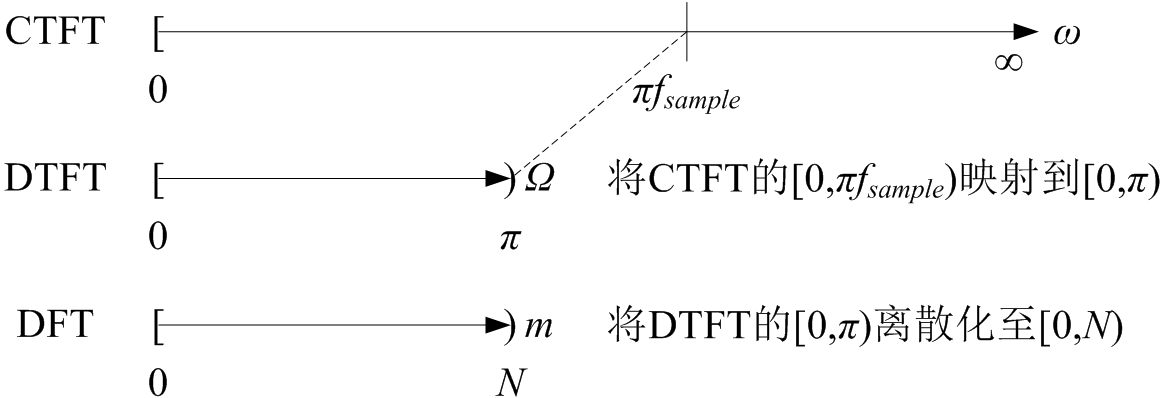
\includegraphics[height=3cm]{6.3.6-1.png}
\end{figure}

{\bf 采样频率$f_{sample}$的影响}

DTFT将CTFT的$0\text{~}\pi \cdot f_{sample}$部分映射到窗口$\left[ 0,\pi \right] $中,所以采样频率决定DTFT能看到多高频率范围,$f_{sample}$越高,越能收集信号的变化,对应地DTFT越能看到高频,越逼近CTFT。

{\bf 采样数量$N$的影响}

DFT再将DTFT的窗口离散化成$\left[ 0,N/2 \right) $,$X\left[ m \right] $的整体包络就是$X\left( \varOmega \right) $,所以信号序列的长度(即$N$)并不改变$X\left[ m \right] $的整体形状,$N$越大,表示对信号收集地越多,DFT越密集、分辨率越高、越细腻,越能精确描述包络形状,越贴近对应的$X\left( \varOmega \right) $曲线。

综合来讲,对于同样的信号,$f_{sample}$决定了你能看到多宽的频率(即频率的上限),$N$决定了你能看到多细腻的频谱,或者说DFT和CTFT的“长相一致程度”。

~

\begin{example}
假设有一个方波信号,前10秒是1,后面都是0,分析不同的采样数量和不同的采样频率对DFT的影响。
\end{example}

信号及其傅里叶变换如下图:
\begin{figure}[h]
\centering
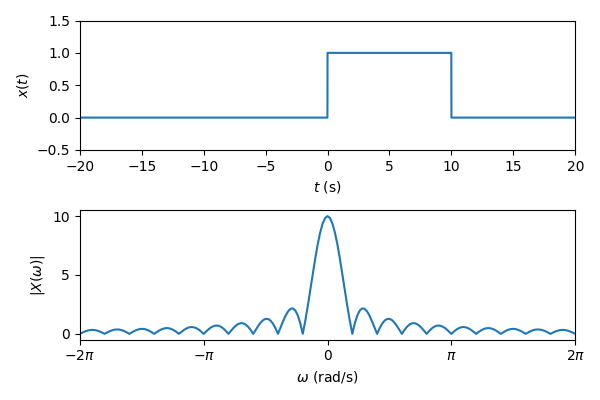
\includegraphics[height=4cm]{6.3.6-2.png}
\end{figure}

先分析不同的采样数量对DFT的影响,假设采样周期1s,即:
\[
x\left[ n \right] =1 \qquad n=0,1,2,3,4,5,6,7,8,9
\]
取三个不同的采样数量(10s,20s,110s),用Python计算DFT并作图:

\begin{python}
n_1  = np.arange(0, 10)
xn_1 = np.ones(10)
Xm_1 = my_dft(xn_1)

n_2  = np.arange(0, 20)
xn_2 = np.where(n_2<10, 1, 0)
Xm_2 = my_dft(xn_2)

n_3  = np.arange(0, 110)
xn_3 = np.where(n_3<10, 1, 0)
Xm_3 = my_dft(xn_3)

axs[0].stem(n_1, np.abs(Xm_1))
axs[1].stem(n_2, np.abs(Xm_2))
axs[2].stem(n_3, np.abs(Xm_3))
\end{python}

\begin{itemize}
    \item 如果采样数量小于等于方波,则这个序列其实可以认为是$x\left[ n \right] =1$,DFT也说明了这个问题;
    \item 采样数量越多,越能说明原连续信号,DFT的结果约贴近CTFT,结合量纲分析,就是频谱的分辨率更高。
\end{itemize}

\begin{figure}[ht]
\centering
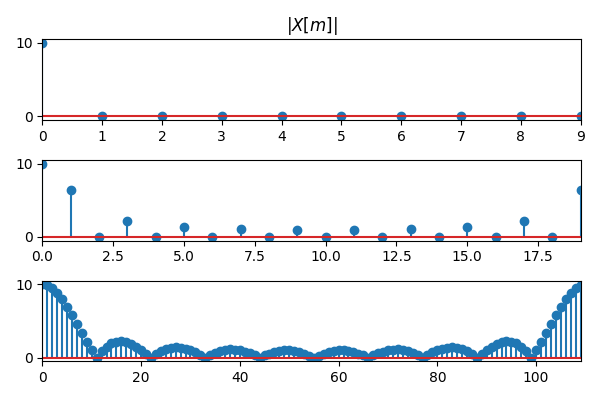
\includegraphics[height=5cm]{6.3.6-3.png}
\end{figure}

再分析采样频率对DFT的影响,分别用三种不同的采样频率(1s,0.5s,0.2s),采样数量都为50s,用Python计算DFT并作图:

\begin{python}
n_1  = np.arange(0, 50)
xn_1 = np.where(n_1<10, 1, 0)
Xm_1 = my_dft(xn_1)

n_2  = np.arange(0, 100)
xn_2 = np.where(n_2<20, 1, 0)
Xm_2 = my_dft(xn_2)

n_3  = np.arange(0, 250)
xn_3 = np.where(n_3<50, 1, 0)
Xm_3 = my_dft(xn_3)

axs[0].plot(n_1, np.abs(Xm_1))
axs[1].plot(n_2, np.abs(Xm_2))
axs[2].plot(n_3, np.abs(Xm_3))
\end{python}

\begin{figure}[h]
\centering
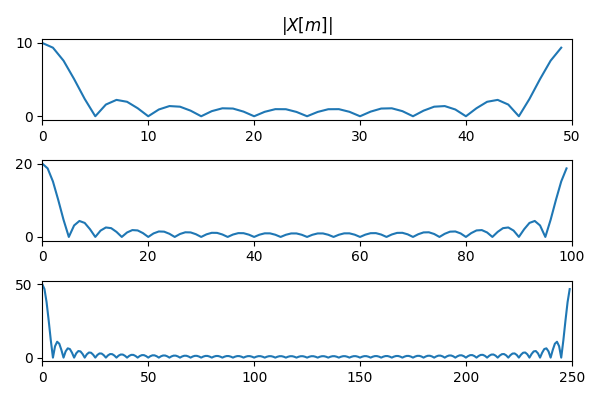
\includegraphics[height=5cm]{6.3.6-4.png}
\end{figure}

\begin{itemize}
    \item 为了看清,使用plot函数作图;
    \item 采样频率影响DFT的大致形状;
    \item 采样频率不影响lobe的“宽度”(即DFT两个相邻0值的间隔距离),影响lobe的“厚度”;
    \item 采样频率越高,频率范围越“拥挤”,即可看到的频率越多,结合量纲分析就是越能看到高频部分;
    \item 采样频率越高,DFT低频份量占比越多,这和采样周期对DTFT的影响的分析一致。
\end{itemize}

%============================================================
\subsection{填充技术对DFT的影响}

虽然采样数量越多,DFT越能体现CTFT,但真实系统对采样数量还是有要求的,采样数量不可能无限多。
这里讨论一种填充技术,书中称为“DFT of truncated signal”。

如下连续信号,以$T=0.5$采样,信号及其傅里叶变换如下:
\begin{align*}
&x\left( t \right) =0.9^t \qquad t\geqslant 0 \\
&X\left( \omega \right) =-\frac{1}{\ln 0.9-i\omega}
\end{align*}
\begin{figure}[h]
\centering
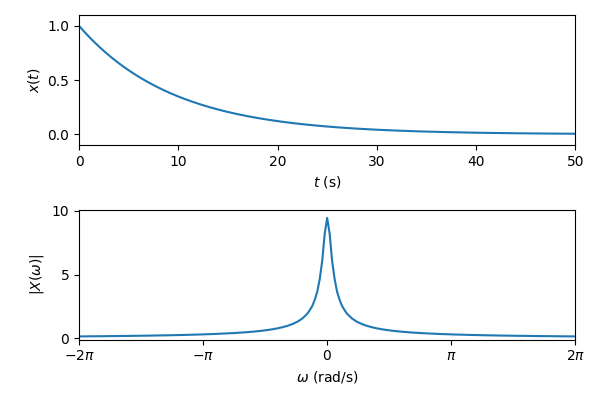
\includegraphics[height=4cm]{6.3.7-1.png}
\end{figure}
% \begin{figure}[h]
% \centering
%     \begin{minipage}{0.48\linewidth}
%     \centerline{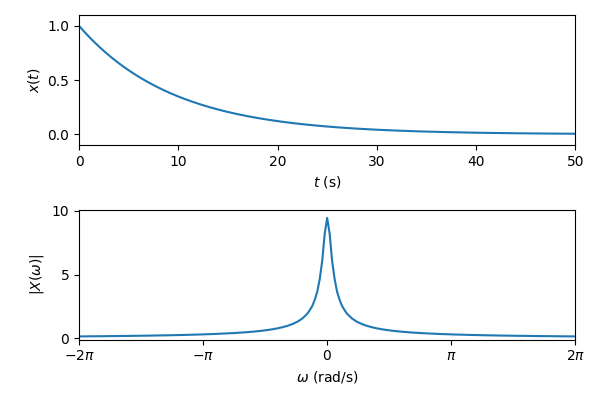
\includegraphics[height=4cm]{6.3.7-1.png}}
%     \end{minipage}
% \hfill
%     \begin{minipage}{0.48\linewidth}
%     \begin{align*}
%     &x\left( t \right) =0.9^t \qquad t\geqslant 0 \\
%     &X\left( \omega \right) =-\frac{1}{\ln 0.9-i\omega}
%     \end{align*}
%     \end{minipage}
% \end{figure}

使用Python辅助分析:
\begin{python}
n_1  = np.arange(0, 30, 0.5)
xn_1 = 0.9**n_1
Xm_1 = my_dft(xn_1)

n_2  = np.arange(0, 10, 0.5)
xn_2 = 0.9**n_2
Xm_2 = my_dft(xn_2)

n_3  = np.arange(0, 30, 0.5)
xn_3 = 0.9**n_3; xn_3[xn_2.size:] = 0
Xm_3 = my_dft(xn_3)

axs[0].plot(np.abs(Xm_1))
axs[1].plot(np.abs(Xm_2))
axs[2].plot(np.abs(Xm_3))
\end{python}

\begin{itemize}
    \item 足额采样,xn\_1采样前30s,DFT结果Xm\_1大致能体现CTFT,如下第一幅;
    \item 采样不足,xn\_2只采样前10s,DFT结果Xm\_2开始有明显失真,如下第二幅。
    \item 填充技术弥补采样不足,xn\_2只采样前10s,后20s人为填充0,相当于时域叠加了方波,DFT结果Xm\_3叠加了sinc函数,如下第三幅。
\end{itemize}

\begin{figure}[h]
\centering
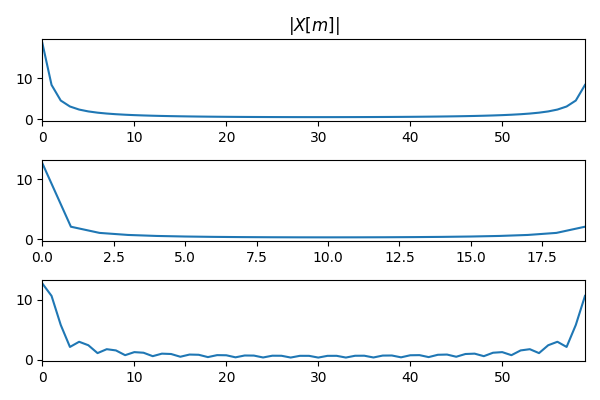
\includegraphics[height=5cm]{6.3.7-2.png}
\end{figure}

填充技术其实是一种“伪细腻化”技术,填充的值越接近实际信号,越接近真实的细腻。




